\begin{figure}[!h]
    \centering
    \begin{subfigure}{.5\textwidth}
      \centering
      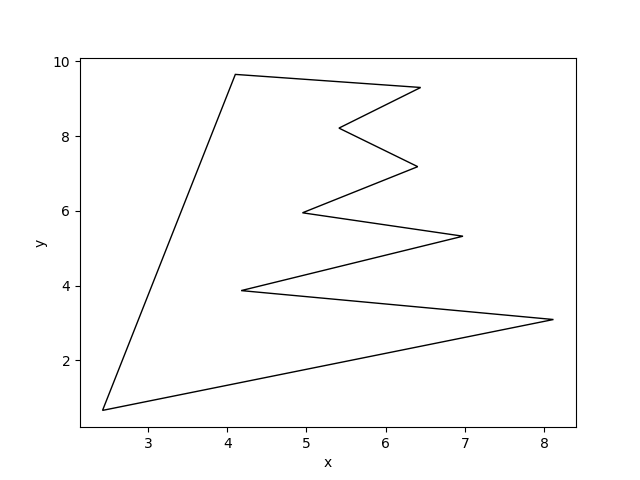
\includegraphics[width=.9\linewidth]{polygon_5.png}
      \caption*{Rys. 1: Wielokąt z wykładu.}
      \label{fig:sub1}
    \end{subfigure}%
    \begin{subfigure}{.5\textwidth}
      \centering
      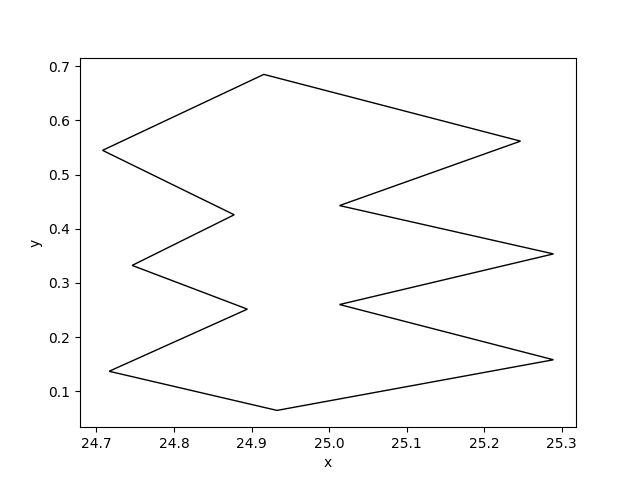
\includegraphics[width=.9\linewidth]{christmas_tree.png}
      \caption*{Rys. 2: Choinka.}
      \label{fig:sub2}
    \end{subfigure}
    \label{fig:test}
    \end{figure}

\newpage

    \begin{figure}[!h]
    \centering
    \begin{minipage}{.5\textwidth}
      \centering
      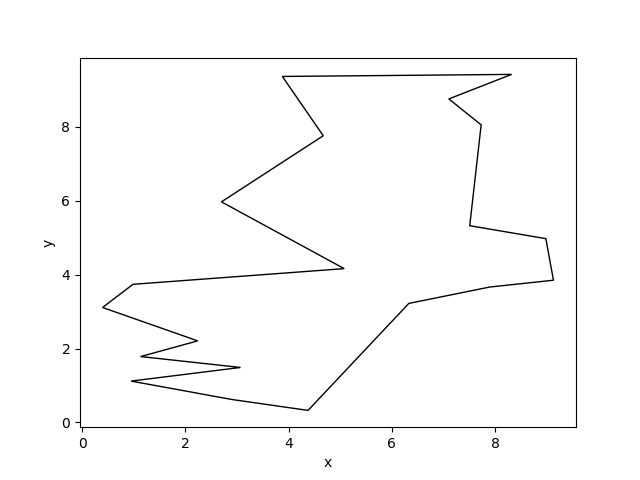
\includegraphics[width=.9\linewidth]{polygon_weird.png}
      \caption*{Rys. 3: Wielokąt 1.}
      \label{fig:test1}
    \end{minipage}%
    \begin{minipage}{.5\textwidth}
      \centering
      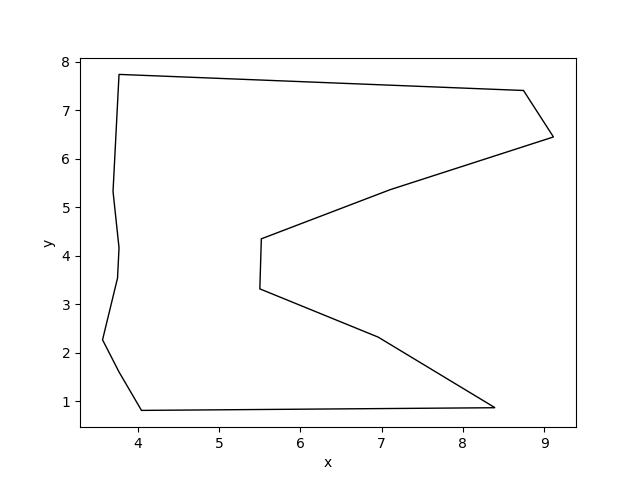
\includegraphics[width=.9\linewidth]{polygon_weird_2.png}
      \caption*{Rys. 4: Wielokąt 2.}
      \label{fig:test2}
    \end{minipage}
    \end{figure}
    \begin{figure}[!h]
        \centering
        \begin{minipage}{.5\textwidth}
          \centering
          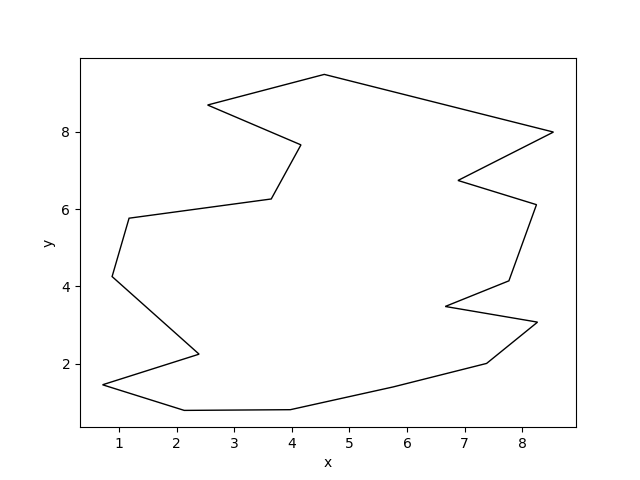
\includegraphics[width=.9\linewidth]{polygon_weird_3.png}
          \caption*{Rys. 5: Wielokąt 3.}
          \label{fig:test1}
        \end{minipage}%
        \begin{minipage}{.5\textwidth}
          \centering
          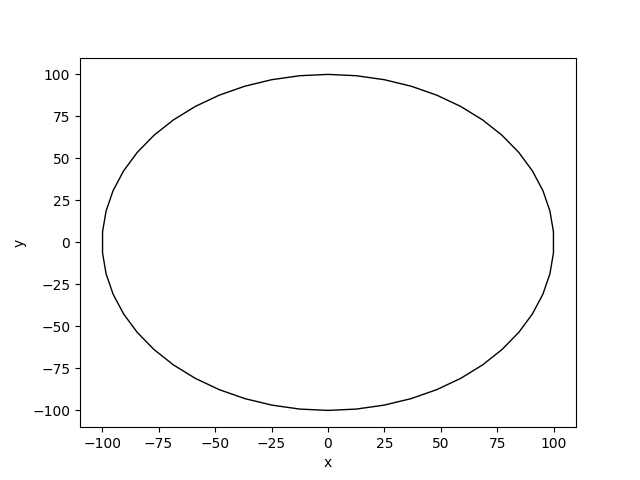
\includegraphics[width=.9\linewidth]{polygon_50.png}
          \caption*{Rys. 6: 50-kąt foremny.}
          \label{fig:test2}
        \end{minipage}
        \end{figure}

  \subsection{Dalczego wybraliśmy te zbiory testowe}
  \begin{enumerate}
    \item Wielokąt z wykładu to wielokąt wklęsły, który wykorzystujemy do sprawdzenia czy nasz alogrytm dobrze sprawdza czy odcinek pomiędzy wierzchołkami jest zawarty w wielokącie.
    \item Choinka to przykład wielokąta, który ma wierzchołki naprziemiennie z różnych łańcuchów oraz jest wielokątem wklęsłym, co pozwala na testowanie czy nasz algorytm dobrze sprawdza czy przekątna poprowadzona między wierzchołkami leży wewnątrz wielokąta.  
    \item Wielokąt 1 to losowy, skomplikowany, wklęsły wielokąt.
    \item Wielokąt 2 to losowy, skomplikowany, wklęsły wielokąt.
    \item Wielokąt 3 to losowy, skomplikowany, wklęsły wielokąt.
    \item 50-kąt foremny - przypadek ekstremalny dla wielokąta w którym wierzchołki naprzemian są z lewego i prawego łancucha.
  \end{enumerate}